\section{System Model}\label{sec_system}
Figure~\ref{fig_system} illustrates the system model in consideration which consists of AUTOSAR software applications \ttsexp{A}{a} partitioned on an execution platform \tteP, where  $\sexp{\pN}{n}[h]$ are the computing unit, \ttpB{} is the shared network bus. Each application has user-defined requirement {\sffamily(RL,EE,CL)}, where the tuple elements respectively refer to the reliability goals (or requirement), end-to-end timing requirements and criticality levels. And each computing node has  provisions (or capabilities) {\sffamily(HZ,PW,FR)}, where the tuple elements respectively refer to the processor speed, power-consumption specifications and failure rates.
 \begin{figure}[!h]
	\centering
	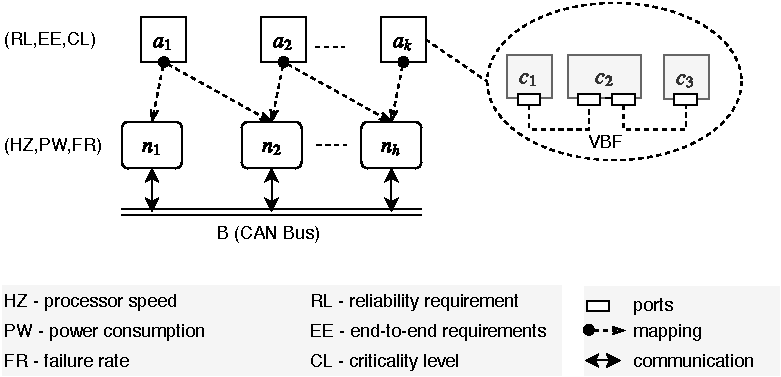
\includegraphics[scale=0.8]{system_model2}%softwareallocation
	\caption{System Model.}
	\label{fig_system}
\end{figure}

\paragraph{Notations} For easy reading, we introduce the main notations used throught the paper as shown in Table~\ref{tbl_notations}.
\begin{table}[h]
\centering\small
\begin{tabular}{@{}lp{0.55\textwidth}@{}}
\toprule
Notation & Description\\
\midrule
\multicolumn{2}{l}{$\bullet$ Related to software applications}\\
\ttsexp{A}{a}    		             & AUTOSAR software applications*\\
$\ar=\langle V,E,w\rangle$    		                     & a software application, modeled as directed acyclic graph of runnables\\
$\mathcal{V}(\ar)\in \ssb{R},\mathcal{E}(\ar)$  & nodes and links of \ttar, respectively\\
\ttsexp{\Gamma}{\Gamma}  & paths of \ttar{} and denote end-to-end chains\\[6pt] \hline 

\multicolumn{2}{l}{$\bullet$ Related to software components}\\
\ttsexp{C}{c}     		             & software-component types used in \ttar\\
\sexpsb{Q}{q}    		            & component replicas of type \ttssb{c}\\
\sexpsb{R}[i]{r}[j]   	             & runnables of \ttssb{c}\\[6pt]\hline 

\multicolumn{2}{l}{$\bullet$ Related to the execution platform}\\
\ttsexp{N}{n}         	            & computation (or computing) nodes      \\
$B$        	           & the shared network bus\\[6pt]\hline 

\multicolumn{2}{l}{$\bullet$ Related to the mapping}\\
\sexpsp{\textbf{x}}{\textbf{x}}         & a mapping vector from \ttssp{Q} to $N$             \\
\ttxkij & the mapping of \ttssb{c} to $n_l$, where $l=\xkij$\\
\ttat    		                     & a software application, modeled as directed acyclic graph of tasks, refines \ttar \\
\sexpsb{T}[i]{\tau}[j]   	             & tasks mapped to \ttssb{c}\\[6pt]\hline 
\multicolumn{2}{l}{$\bullet$ Related to the optimization}\\
$Power(\textbf{x})$                		& total power consumption of  $A$ in \ttx    \\
$Reliability_{a}(\x)$      					& application reliability  of $a\in A$ in \ttx              \\
$ResponseTime_{\tau}(\x)$     		& response time of  $\tau \in V(\ssb{g}[\tau])(\x)$                       \\
$Delay_\gamma(\x)$            			& age delay of $\gamma \in \ssp{\Gamma} $   in \ttx     \\
\bottomrule
\end{tabular}
\caption{The Main Notations Used Throughout the Paper. \\
{\footnotesize * Note: the total elements in a set $S$ is denoted by \ttn{S}, e.g., \ttn{A} denotes the number of applications in the set $A$, essentially it refers to cardinality of the set.}}
\label{tbl_notations}
\end{table}
\subsection{Software Applications}
A software application represents an independent and self-contained user-defined software functionality, e.g., x-by-wire, electronic throttle control, and flight control. In AUTOSAR, software applications are developed using AUTOSAR \textit{Software Component} (SWC), which is a design-time concept that represents the lowest-level hierarchical element in the software architecture of the application, therefore, a software component is atomic, hence is mapped to a single computing unit. The software component is implemented by the AUTOSAR runnables and contains the timing specifications and computation resources needed by the runnables. We formally represent the AUTOSAR software application as follows:
\begin{definition}[AUTOSAR Software Application\footnote{ Note: only relevant concepts of the official AUTOSAR software application definition is assumed to avoid unnecessary complexity. }]\label{def_application}We represent the AUTOSAR software application as a \textit{directed acyclic vertex-weighted} graph $\langle V, L, w\rangle$ of periodic runnables, where $V$ denotes runnable nodes, $a_{ij}\in L$ a data-dependency link from $r_i$ to $r_j$, where $i \neq j$. The assignment function $w: V\rightarrow (\mathrm{E}_i\mathrm{,D,P, N})$ sets each runnable nodes the computation cost such as worst-case execution times (WCET) $\mathrm{E=\{E}_h:h=1,...,n_N\}$, deadline D and period P, where $\mathrm{E}_h\in \mathrm{E}$ is the WCET of $r$ on the computing unit $n_h\in N$.
\end{definition}
\begin{figure}
	\centering
	\begin{minipage}{.45\textwidth}
		\centering
	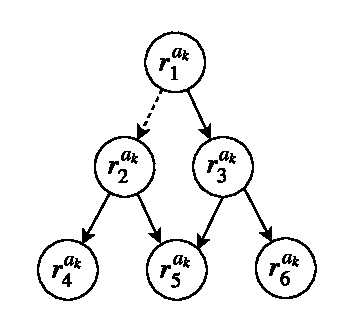
\includegraphics[width=0.7\linewidth]{img/dag_runnables}
	\caption{Software Application Example, Modeled as DAG of Runnables.}
	\label{fig_dag_runnables}
	\end{minipage}\hfill
	\begin{minipage}{0.45\textwidth}
		\centering
		\begin{tabular}{@{}llll@{}}
		\toprule
		\ttssb{c}& \ttssb{r}[j] &$(\mathrm{E}_h, \mathrm{P=D})$ & $\prec$ \ttssb{r} [i]\\ \midrule
		1&1 & $(0.1,10)$   & 2 \\ 
		2&2 & $(0.1,20)$ &  \\ 
		2&3 & $(0.1,15)$ &  \\ 
		2&4 & $(0.1,8)$   &  \\ 
		3&5 & $(0.1,12)$  &  \\ 
		3&6 & $(0.1,6)$   &  \\ 
		\bottomrule 
		\end{tabular}
		\captionof{table}{Timing Specifications  of the Runnables from Figure~\ref{fig_dag_runnables}}
		\label{tbl_dag_runnables_specs}
	\end{minipage}
\end{figure}

A path in the graph $\ssb{\Gamma}[l]=\ssb{r}\rightarrow,...,\rightarrow,\ssb{r}[j]$ represents a \textit{cause-effect} chain, where $\ssb{r},\ssb{r}[j]\in \mathcal{V}(\ar)$ are source and sink of the chain, e.g., in the application \ttar[1] in Figure~ \ref{fig_dag_runnables}, $\ssb{r}[1]\rightarrow \ssb{r}[3]\rightarrow \ssb{r}[5]$ is the chain, and $\ssb{r}[1],\ssb{r}[5]$, respectively are the source and the sink of the chain. A chain is a subfunctionality of the application that is triggered by a stimulus (or stimuli), e.g., pressing a brake pedal, and the corresponding response to actuate the vehicle braking to the desired speed level. It usually has a user-defined timing requirement, known as \textit{end-to-end} timing requirement (EE), which puts an upper-bound on the duration between the stimulus and the corresponding response of executing the chain. The set of chains are represented as \ttsexp{\Gamma}{\Gamma}. Note:  each runnable is subscribed  to at least one chain.

\subsection{Scheduling Software Applications}
We assume software applications share the execution platform such as the computing units and the on-board network bus, following the mixed-criticality design~\cite{Vestal2007PreemptiveAssurance}. Thus, software applications with different software criticality should be isolated in order to prevent interference of lower-criticality applications on the higher-critical applications. For example the brake-by-wire system realizes a safety-criticality functionality, and is distributed over multiple computing units. Another application with infotainment functionality also shares the units. The mixed-criticality design ensures that both applications are schedulable during absence of errors, however, the braking application must also be schedulable in cases of overrun due to errors, e.g., by degrading or halting the infotainment application. There are several techniques in the literature that deal with the scheduling of mixed-criticality applications on \textit{uniprocessor} systems \cite{Vestal2007PreemptiveAssurance}. In this work, we consider the \textit{partitioned criticality (PC)} (or criticality-as-priority assignment, CAPA) technique to schedule the mixed-criticality applications, which prioritizes applications based on criticality, rather than \textit{deadline} as used by the deadline monotonic assignment \cite{Baruah2011Response-timeSystems}. In contrast to other techniques, CAPA is easy to implement and does not require runtime monitoring, e.g., using servers \cite{AbeniIntegratingSystems,Ashjaei2017DesigningSystems,Inam2014ThePlatforms}, though not efficient\footnote{Note: scheduling techniques other than the PA technique can be used with our approach to schedule the applications.}. Thus, the software  applications are schedulable according to CAPA if the runnables, messages, and chains in the applications are schedulable, that is, they meet their corresponding deadlines. 

Next, we explain the mapping rules applied in this work.

\subsubsection{Runnables-to-Tasks Mapping/Transformation}\label{subsec_runnables-to-tasks}
In the mapping process, one or more runnables can be merged to optimize the runtime execution by reducing the number of tasks scheduled by the OS. In this work, we merge the runnables $a,b\in \gr{V}{\ar}$ into the task $v\in \gr{V}{\at}$ if the following two conditions are satisfied:
\begin{enumerate*}[label=(\roman*)]
	\item $(a,b)\in \mathcal{E}(\ar)$ is a link in the graph,
	\item the period of $a$ is a factor of $b$, or vice versa
\end{enumerate*}, otherwise, each runnable is mapped to a separate task, inheriting the timing specifications of the runnable.
If the merging conditions are met, the timing specifications of $v$ are set as follows: 
\begin{enumerate*}[label=(\roman*)]
	\item the WCET of the task is set to the sum of the WCET of the runnables, i.e., E$_h^v=$E$_h^a + $E$_h^b$, for all $h:1,...,n_N$,
	\item the period and deadline of the task is set to the minimum of the runnables' periods, P$_v$=D$_v=min($P$_a, $P$_b)$
\end{enumerate*}
% \begin{figure}
%     \centering
%     \begin{subfigure}[b]{0.3\textwidth}
%         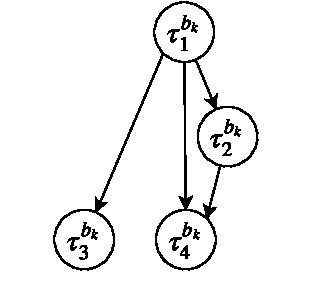
\includegraphics[width=\textwidth]{img/dag_tasks}
%         \caption{A Software Application Modeled as Directed Acyclic Graph.}
%         \label{fig:gull}
%     \end{subfigure}
%     ~ %add desired spacing between images, e. g. ~, \quad, \qquad, \hfill etc. 
%       %(or a blank line to force the subfigure onto a new line)
%     \begin{subfigure}[b]{0.3\textwidth}
%         \includegraphics[width=\textwidth]{tiger}
%         \caption{A tiger}
%         \label{fig:tiger}
%     \end{subfigure}
%     ~ %add desired spacing between images, e. g. ~, \quad, \qquad, \hfill etc. 
%     %(or a blank line to force the subfigure onto a new line)
%     \begin{subfigure}[b]{0.3\textwidth}
%         \includegraphics[width=\textwidth]{mouse}
%         \caption{A mouse}
%         \label{fig:mouse}
%     \end{subfigure}
%     \caption{Pictures of animals}\label{fig:animals}
% \end{figure}

\begin{figure}
\vspace{0pt}\raggedbottom
	\begin{minipage}{.475\textwidth}
		\centering
		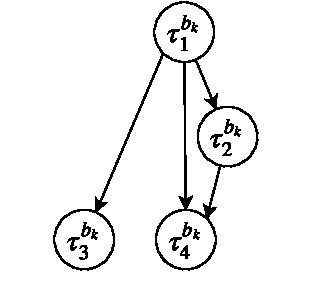
\includegraphics[width=0.6\linewidth]{img/dag_tasks}
		\caption{A Software Application Modeled as Directed Acyclic Graph.}
		\label{fig_dag_tasks}
	\end{minipage}%
\hfill
	\begin{minipage}{0.475\textwidth}
	\centering
		\begin{tabular}{@{}lll@{}}
						&&\\
			&&\\
			\toprule
			\ttssb{\tau}&$\bigcup\ssb{r}[j]$&$(\mathrm{E}_h, \mathrm{P=D})$ \\ 
			\midrule
			1 & 1,2 &  $(0.2,10)$\\ 
			2& 3 &  $(0.1,15)$\\ 
			3& 4&  $(0.1,8)$\\ 
			4 & 5,6 &  $(0.1,6)$\\ 

			\bottomrule 
		\end{tabular}
		\caption{Tasks Timing Specifications after Merging.}
		\label{tbl_tasks_specs}
	\end{minipage}
\end{figure}


The AUTOSAR software applications is shedulable if and only if its task graph is schedulable, that is each task node meets its deadline, each communication between task nodes (that is, the message) meets its deadline, and the chain meets end-to-end requirement. The schedulability analysis of the tasks, messages and chains used in this work are explained next.

\subsubsection{Scheduling of Tasks and Messages}\label{subsec_response-time_analysis}
Following the CAPA scheduling technique, the tasks in the distributed system are assigned priorities according to their criticality, thus the higher the application's criticality, the higher the priority that its tasks acquire
\[
cri(b_i)>cri(b_j)\implies \forall \tau_1,\in V(b_i)\forall \tau_2\in V(b_j)\ Pri(\tau_1)>Pri(\tau_2),
\]
where $\forall i,j:1,...,n_A\land i\neq j$, $cri$ and $pri$ are predicates which determine the criticality and priority of tasks $\tau_1,\tau_2$, respectively; $\mathcal{V}(b_i) and \mathcal{V}(b_j)$ return the tasks of $b_i$ and $a_j$, respectively.

The tasks are scheduled using the \textit{fixed-priority preemptive scheduling policy} (FPPS)~\cite{Sha2004RealPerspective}, and the schedulability analysis is conducted via the classical response-time analysis (RTA) as shown by Equation~(\ref{eqn_responsetimeanalysis}) \cite{Baruah2011Response-timeSystems}. The task $\tau$ is schedulable if the response time of a task $\delta_\tau$ is less than or equal to its deadline \ttDL, i.e., tasks a $\delta_\tau\leq \DL_\tau$. The

\begin{align}
\label{eqn_responsetimeanalysis}
R_\tau=C_\tau+\sum_{j\in h\!p(\tau)}
{
	\ceil[\Big]
	{
		\frac{R_\tau}{P_j}
	}C_j
},
\end{align}
where $C_\tau,C_j$ are execution times of the lower and higher priority tasks, respectively; $h\!p(\tau)$ is the predicate that returns the higher-priority tasks than $c_\tau$.

The messages in the CAN bus are scheduled using the fixed, non-preemptive scheduling policy. Similar to the tasks, the priority of messages follows the CAPA technique to achieve the mixed-criticality requirement. This can easily be achieved by inheriting the priority of each sender task communicating over the bus $pri(m)$ to the successor message $suc(\tau)$, that is $pri(m)=pri(\tau)|\tau = suc(m)$. The schedulability of messages is checked using the classical response-time analysis of the CAN network using Equation~(\ref{eqn_responsetimeanalysisCAN}), as presented by Rob Davis et. al~\cite{Davis2007ControllerRevised}. The worst-case response time of a message is computed as the sum of its \textit{jitter} (that is, the time  taken by the sender task to queue for transmission) $J_m$, the \textit{interference} time (that is, the message delay in the queue) $w_m$, and its \textit{transmission} time  (that is, the longest time for the message to be transmitted) $c_m$ over the network.
\begin{align}
\label{eqn_responsetimeanalysisCAN}
R_m&=J_m+w_m+c_m\\
\label{eqn_interference}
w_m&=B_m+
\sum_{\forall k\in hp(m)}
{
	\ceil[\Big]
	{
		\frac{w_m+\tau_{bit}}{P_k}
	}c_k
}\\
\label{eqn_iblocking}
B_m&=\max_{\forall k\in lp(m)}(c_k),
\end{align}

Note: we assume no jitter, therefore, the interference formula is reduced as shown in Equation (\ref{eqn_interference}), where $B_m$ is the blocking time caused by the lower-priority messages using the CAN bus (since it is non-preemptive) and is computed by Equation (\ref{eqn_iblocking}); $hp(m)$ finds the set of higher-priority messages, which interfere with the transmission of the message $m$.

\subsubsection{Scheduling Cause-effect Chains}\label{subsec_cause-effect_chains}
The chain consists of independently clocked tasks, which results in undersampling/oversampling effects. As a result, a data that propagates across the chain is characterized by having various delays, which are discussed in detail by Feiertag et al.~\cite{Feiertag2009ASemantics} in the context of single-register buffer communication,  which is a common practice in control systems design, e.g., automotive software applications~\cite{Becker2017End-to-endSystems}. In this work, we demonstrate the two widely used semantics in the automotive domain: \textit{age} delay and \textit{reaction} delay, and consider only the age delay in the analysis. The age delay is the time elapsed between the data arriving a the input register (which is the stimulus) and its corresponding latest, non-overwritten output (response) at the output register. And, the reaction delay is the earliest time the system takes to respond to a stimulus that ``just missed" the read access at the input of the chain.

Consider the chain $\tau_1\rightarrow \tau_2\rightarrow \tau_4$ in the task graph from Figure~\ref{fig_dag_runnables}. Assume the chain is mapped to the computing units $n_1$ and $n_2$ as illustrated in Figure~\ref{fig_cause_effect_chain}, and that the tasks in the chain communicate using the single-register buffers. The tasks $\tau_1$ and $\tau_4$ execute on node $n_1$, whereas, task $\tau_2$ executes on node $n_2$. The input data can arrive at any time in the input register {\sffamily IR}. 
\begin{figure}
	\centering
	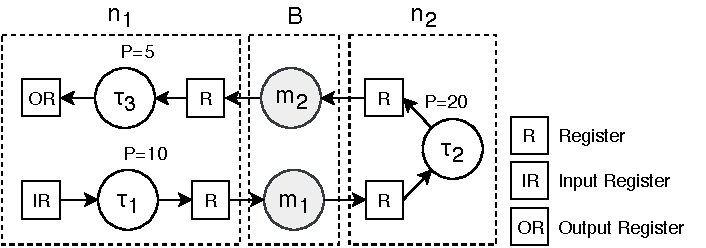
\includegraphics[width=0.7\linewidth]{img/cause_effect_chain_ntk}
	\caption{A Cause-effect Chain, mapped on nodes $n_1$ and $n_2$.}
	\label{fig_cause_effect_chain}
\end{figure}

The execution behavior of the chain is illustrated in Figure~\ref{fig_timedchainntk} over two hyper-periods.  Note that, the message between $\tau_2$ and $\tau_3$ is not shown in the figure for simplicity. The red inverted arrows in the figure represent the reading of data from the input register, whereas the dashed-line arrows represent the timed paths through which the data propagates from the input to the output of the chain. Thus, the age delay is the time elapsed between the $3^{rd}$ instance of  $\tau_1$  and the $10^{th}$ instance of $\tau_3$. The timing constraint corresponding to the age delay is frequently used in the control systems where freshness of data is paramount, e.g., braking a car over a bounded time. Assume that data arrives just after the start of the $1^{st}$ instance of $\tau_1$ execution. The data corresponding to this event is not read by the current instance of $\tau_1$. In fact, the data will be read by the $2^{nd}$ instance of $\tau_1$. The earliest effect of this data at the output of the chain will appear at the $7^{th}$ instance of $\tau_3$, which represents the reaction delay. This delay is useful in the body-electronics domain where first reaction to events is important, e.g., in the button-to-reaction applications. For detailed discussion of the different delay semantics, we direct the reader to check research work by Mubeen et al.~\cite{Mubeen2019SupportingConstraints}. 
\begin{figure}[h]
	\centering
	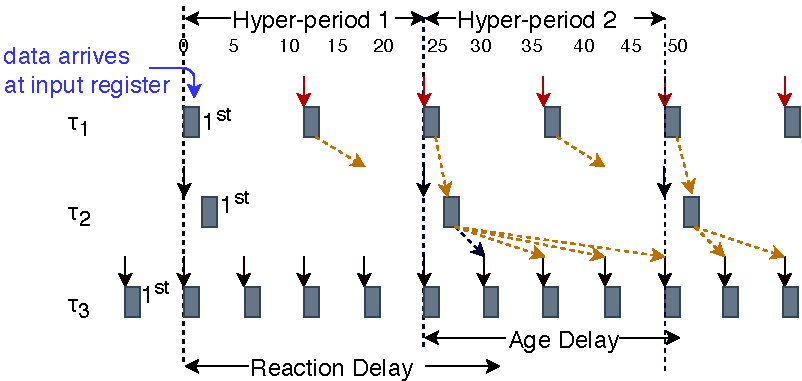
\includegraphics[width=0.8\linewidth]{img/timedchain_ntk}
	\caption{Reaction and Age Delays in the Cause-effect Chain, Shown in Figure {\ref{fig_cause_effect_chain}}.}
	\label{fig_timedchainntk}
\end{figure}

Thus, if the chain is mapped to a single computing unit, the age delay  $\Delta^{sub}$ is computed using Equation (\ref{eqn_agedelay_singlenode}), that is by taking the difference between the activation of the sink and the source tasks, plus the response-time of the sink task. Otherwise, if it is mapped to multiple units and the bus, the delay $\Delta$ is computed compositionally by identifying the subchains using Equation (\ref{eqn_agedelay_multinode}). In the latter case, the response-time of messages $\delta^{msg}$, and the ``just missed'' case that is by adding the period of the successor task $P_{suc(j)}$ are  taken into consideration.
\begin{align}
	\label{eqn_agedelay_singlenode}
	\Delta^{sub}(\gamma) &= \alpha(sin(\gamma))-\alpha(src(\gamma)) + \delta(sink(\gamma)) & \text{single unit}\\
	\label{eqn_agedelay_multinode}
	\Delta(\gamma)&=\sum_{i\in I_{\gamma}}{\Delta^{sub}(i)} + \sum_{j\in  J_{\gamma}}{[\delta^{msg}(j)+P_{suc(j)}]}, &\text{multiple units}
\end{align}
where $\alpha(\tau)$ computes the activation of the task $\tau$, based on the age-delay semantics.

\subsection{Reliability of Software Applications}\label{sub_reliability}
In this context, \textit{software application reliability} refers to the probability that a software application functions correctly by the time $t$, or within the time interval $[0, t]$ \cite{Goel1985SoftwareApplicability}. Redundancy is the most common way of implementing fault tolerance and increasing the reliability of a system. Redundancy can be implemented according to different schemes such as hot stand-by, cold stand-by, etc.~\cite{Dubrova2013Fault-tolerantDesign}, which differ on the number of replicas that are active as well as the methods for detection and compensation of faulty replicas. In our system model, we consider the hot-standby scheme, where replicated components maintain the same state, but only one replica (the so-called \textit{primary}) effectively acts on the environment, for instance to issue an input. In the software application $A_k$, the primary software component is denoted as \ttssb{q}[i,1], whereas the secondary software component, which is in the stand-by is identified, by \ttssb{q}[i,2].

In this work the details of the redundancy scheme are abstracted away under the following assumptions:
\begin{enumerate}[label=(\roman*)]
    \item Software does not contain design errors. This has two implications: first, that hardware elements, i.e. computing nodes and communication buses, are the only causes of failure and, second, that introduction of N-version programming is not required. Different replicas of the same software component execute exactly the same program.
	\item Hot stand-by redundancy (also known as Primary/backup) is used for detection and replacement of failed components.
	\item Software components need to be replicated only if the application's reliability requirement is not met without replication, otherwise they are not replicated.
	\item The time needed to detect and replace a faulty component is considered negligible and will not be taken into account in the response time analysis of tasks and the delay calculation of cause-effect chains;
	\item Because of its simplicity, the mechanism for detection and replacement of faulty components will be considered fault-free, and therefore, it will not be included in the reliability calculations.
\end{enumerate}

Note that, under these assumptions, the reliability of a software application is equivalent to the reliability of the platform on which it is deployed. The reliability of a computing unit (and of the bus) can be easily calculated as $e^{\lambda t}$, where $\lambda$ is an exponentially distributed failure-rate. However, calculating the reliability of the whole execution platform is not trivial for the case with replication. In particular, the traditional series-parallel reliability approach cannot be applied because of the \textit{functional} inter-dependencies created between computing nodes as the result of replication and allocation. To illustrate the complexity, let us assume a software application $A_k$, having  component configurations without and with replication as shown in  Table~\ref{fig_depwor} and~\ref{fig_depwr}, respectively, where $\ssb{q}[i,j]$ is the $j^{th}$ software component replica of software component type $\ssb{c}\in \ssb{C}$. Note: the superscript $k$ is not used for sake of readability.
\begin{table}
	\begin{subfigure}{.5\textwidth}
		\centering
		\begin{tabular}{ccc}
			$n_1$ & $n_2$ & $n_3$\\
			\hline
			\ttssb{q}[1,1]&\ttssb{q}[2,1]& \\
			\ttssb{q}[3,1]& & \\
			\hline
		\end{tabular}	
		\caption{Without Replication.}
		\label{fig_depwor}
	\end{subfigure}%
	\begin{subfigure}{.5\textwidth}
		\centering
		\begin{tabular}{ccc}
			$n_1$ & $n_2$ & $n_3$\\
			\hline
			\ttssb{q}[1,1]&\ttssb{q}[2,1]& \ttssb{q}[2,2]\\
			\ttssb{q}[3,1]& \ttssb{q}[1,2]& \ttssb{q}[3,2]\\
			\hline
		\end{tabular}
		\caption{With Replication.}
		\label{fig_depwr}
	\end{subfigure}%
	\caption{Allocation of the software components.}
	\label{fig_deployment}
\end{table}

The reliability of the software application without replication forms a series path, indicated by the reliability block diagram (RBD) of Figure~\ref{fig_rbd}a. Hence, it is computed as a product of the reliability of $n_1,n_2$ and $B$. However, with replication, two computing nodes can form series and parallel to service the software application,  e.g., due to \ttssb{q}[1,1] and \ttssb{q}[2,2] or \ttssb{q}[3,2], $n_1$ and $n_3$ making series, and due to \ttssb{q}[3,1] and \ttssb{q}[3,2], the nodes make parallel, to realize a partial functionality of the application. In this case, the series-parallel diagram depicted in Figure~\ref{fig_rbd}b does not accurately capture the reliability calculation of the application with replication. Note that, the red-line arrows between $n_1$ and $n_3$ indicates the possibility of the computing nodes becoming series. To overcome this problem, we will use an exact technique for reliability calculation based on the enumeration of the different failure states of the computing nodes. That is, the different failure states of the execution platform are enumerated exhaustively, and subsequently, the total probability the software application functions is computed. This technique will be discussed in great detail in Subsection~\ref{subsec_reliability_constraint}.
\begin{figure}
	\centering
	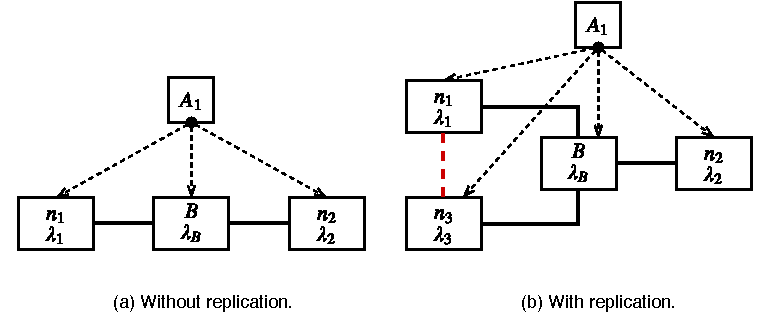
\includegraphics[width=0.8\linewidth]{img/rbd_replication}
	\caption{Reliability Block Diagrams of the Software Application.}
	\label{fig_rbd}
\end{figure}



